\documentclass[12pt, a4paper]{article}

% -----------------------------
% Packages
% -----------------------------
\usepackage{geometry}
\geometry{margin=1in}

\usepackage{fancyhdr}
\usepackage{titlesec}
\usepackage{listings}
\usepackage{xcolor}
\usepackage{graphicx}

% -----------------------------
% Header & Footer
% -----------------------------
\pagestyle{fancy}
\fancyhf{}
\lhead{Kamithkar Vinod}
\rhead{DBT - Assignment 7}
\cfoot{\thepage}

% -----------------------------
% Section Formatting
% -----------------------------
\titleformat{\section}
  {\large\bfseries}
  {Problem \thesection:}
  {0.5em}{}

\titleformat{\subsection}[runin]
  {\bfseries}
  {Code:}
  {0.5em}{}[---]

\titleformat{\subsubsection}[runin]
  {\bfseries}
  {Output:}
  {0.5em}{}[---]

% -----------------------------
% SQL Syntax Highlighting
% -----------------------------
\lstdefinelanguage{SQL}{
  morekeywords={
    SELECT, FROM, WHERE, GROUP, BY, ORDER, ASC, DESC, JOIN, ON, AS,
    AND, OR, NOT, IN, IS, NULL, LIKE, HAVING, COUNT, SUM, AVG, MIN, MAX,
    CREATE, TABLE, INSERT, INTO, VALUES, UPDATE, SET, DELETE, DISTINCT,
    CASE, WHEN, THEN, ELSE, END, BETWEEN, EXISTS, UNION, ALL, ANY, LEFT,
    RIGHT, INNER, OUTER, LIMIT, OFFSET, PROCEDURE, BEGIN, FUNCTION, END,
    RETURNS, RETURN
  },
  sensitive=false,
  morecomment=[l]{--},
  morestring=[b]',
}

\lstset{
  language=SQL,
  basicstyle=\ttfamily\small,
  keywordstyle=\color{blue}\bfseries,
  commentstyle=\color{gray}\itshape,
  stringstyle=\color{red},
  showstringspaces=false,
  frame=single,
  breaklines=true,
  numbers=none
}

% -----------------------------
% Document Start
% -----------------------------
\begin{document}

% -----------------------------
% Title Page
% -----------------------------
\begin{center}
    \LARGE \textbf{Assignment - 7} \\[0.5cm]
    \Large \textbf{Database Management Systems (DBMS)} \\[1cm]

    \begin{tabular}{rl}
        \textbf{Name:} & Kamithkar Vinod \\
        \textbf{Course:} & PG DAC August 2025 \\
        \textbf{PRN:} & 250850320040 \\
        \textbf{Form No:} & 250500480 \\
        \textbf{Date:} & 30-10-2025 \\
    \end{tabular}
\end{center}

\vspace{1cm}
\hrule
\vspace{0.5cm}

% -----------------------------
% Problems Section
% -----------------------------

% Problem 1
\section{Exception Handling}
\textbf{Task:} Create a stored procedure \texttt{add\_department} to insert a department. 
If the department name already exists, handle error 1062 using an \texttt{EXIT} handler 
and display the message "Department already exists".

\subsection{}
\begin{lstlisting}
drop procedure if exists add_department;

delimiter //
create procedure add_department(in dname varchar(50))
begin
    declare exit handler for 1062
    begin
	   select 'Department already exists' as message;
    end;

    insert into departments(dept_name) values (dname);
    select 'Department added successfully' as message;
end //
delimiter ;

call add_department('IT');
\end{lstlisting}

\subsubsection{}
\begin{center}
    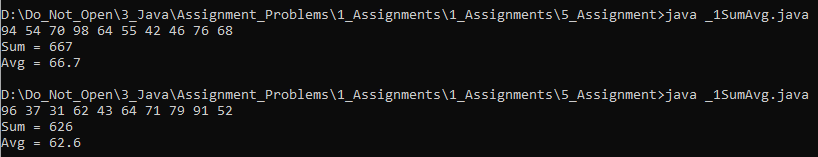
\includegraphics[width=0.8\textwidth]{1.png}
\end{center}

% Problem 2
\section{Exception Handling}
\textbf{Task:} Create a stored procedure \texttt{add\_employee} to insert an employee. 
Handle duplicate employee names using an \texttt{EXIT} handler for error 1062.

\subsection{}
\begin{lstlisting}
drop procedure if exists add_employee;

delimiter //
create procedure add_employee(in name varchar(50), in sal decimal(10, 2), in d_id int)
begin
    declare exit handler for 1062
    begin
	   select 'employee already exists' as message;
    end;
    insert into employees(emp_name, salary, dept_id)
    value (name, sal, d_id);
    select 'employee added successfully' as message;
end //

delimiter ;

call add_employee('Vinod', 43000, 1);
\end{lstlisting}

\subsubsection{}
\begin{center}
    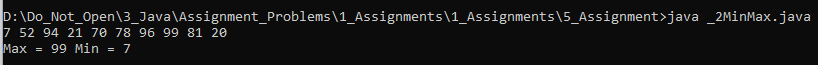
\includegraphics[width=0.8\textwidth]{2.png}
\end{center}

% Problem 3
\section{Exception Handling}
\textbf{Task:} Create a stored procedure \texttt{bulk\_insert\_employees} to insert 5 employees 
in a loop using a \texttt{CONTINUE} handler to skip duplicate names.

\subsection{}
\begin{lstlisting}
drop procedure if exists bulk_insert_employees;

delimiter //
create procedure bulk_insert_employees()
begin
    declare i int default 1;
    declare continue handler for 1062
    begin
	   select concat('Duplicate record found at ', i) as warning;
    end;
    
    while i <= 5 do
        insert into employees(emp_name, salary, dept_id)
        values (concat('Emp', i), 3000*i, 1);
        set i = i + 1;
	end while;
end //
delimiter ;

call bulk_insert_employees();
\end{lstlisting}

\subsubsection{}
\begin{center}
    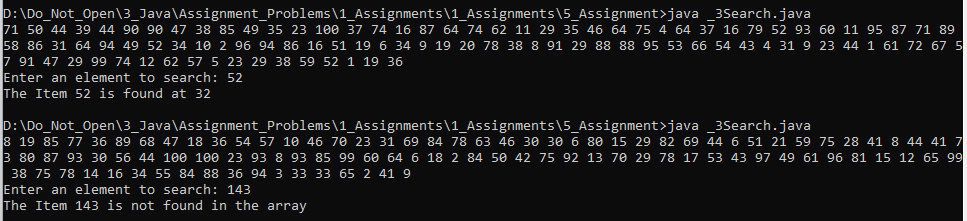
\includegraphics[width=0.8\textwidth]{3.png}
\end{center}

% Problem 4
\section{Exception Handling}
\textbf{Task:} Create a stored procedure \texttt{check\_salary} that checks if a given salary 
is less than 1000. Use \texttt{SIGNAL} to raise a custom error and an \texttt{EXIT} handler to catch it.

\subsection{}
\begin{lstlisting}
DELIMITER //
CREATE PROCEDURE check_salary(IN sal DECIMAL(10,2))
BEGIN
   DECLARE low_salary CONDITION FOR SQLSTATE '45000';
   DECLARE EXIT HANDLER FOR low_salary
   BEGIN
       SELECT 'Salary too low' AS message;
   END;

   IF sal < 1000 THEN
       SIGNAL low_salary;
   ELSE
       SELECT 'Salary acceptable' AS message;
   END IF;
END//
DELIMITER ;

CALL check_salary(800);
CALL check_salary(5000);
\end{lstlisting}

\subsubsection{}
\begin{center}
    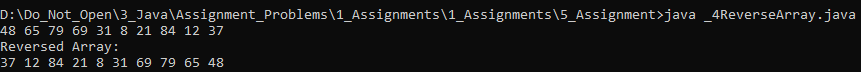
\includegraphics[width=0.8\textwidth]{4.png}
\end{center}

% Problem 5
\section{Exception Handling}
\textbf{Task:} Create a function \texttt{annual\_salary} that returns annual salary as (12 × monthly salary).

\subsection{}
\begin{lstlisting}
DELIMITER //
CREATE FUNCTION annual_salary(monthly DECIMAL(10,2))
RETURNS DECIMAL(10,2)
DETERMINISTIC
BEGIN
   RETURN monthly * 12;
END//
DELIMITER ;

SELECT emp_name, salary, annual_salary(salary) AS yearly FROM employees;

\end{lstlisting}

\subsubsection{}
\begin{center}
    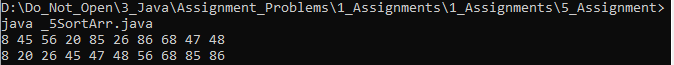
\includegraphics[width=0.8\textwidth]{5.png}
\end{center}

% Problem 6
\section{Exception Handling}
\textbf{Task:} Create a stored procedure \texttt{count\_employees} to count employees 
with non-null department IDs, using a \texttt{CONTINUE} handler to skip null values.

\subsection{}
\begin{lstlisting}
DELIMITER //
CREATE PROCEDURE count_employees()
BEGIN
   DECLARE done INT DEFAULT 0;
   DECLARE total INT DEFAULT 0;
   DECLARE CONTINUE HANDLER FOR NOT FOUND SET done = 1;
  
   SELECT COUNT(*) INTO total FROM employees WHERE dept_id IS NOT NULL;
   SELECT CONCAT('Total employees (with dept): ', total) AS message;
END//
DELIMITER ;

CALL count_employees();

\end{lstlisting}

\subsubsection{}
\begin{center}
    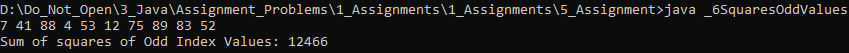
\includegraphics[width=0.8\textwidth]{6.png}
\end{center}

% Problem 7
\section{Exception Handling}
\textbf{Task:} Create a stored procedure \texttt{delete\_employee} that deletes an employee 
based on \texttt{emp\_id}. If the employee is not found, display "No such employee".

\subsection{}
\begin{lstlisting}
DELIMITER //
CREATE PROCEDURE delete_employee(IN eid INT)
BEGIN
   DECLARE EXIT HANDLER FOR SQLEXCEPTION
   BEGIN
       SELECT 'Error deleting employee' AS message;
   END;

   IF (SELECT COUNT(*) FROM employees WHERE emp_id = eid) = 0 THEN
       SELECT 'No such employee' AS message;
   ELSE
       DELETE FROM employees WHERE emp_id = eid;
       SELECT 'Employee deleted' AS message;
   END IF;
END//
DELIMITER ;

CALL delete_employee(10);

\end{lstlisting}

\subsubsection{}
\begin{center}
    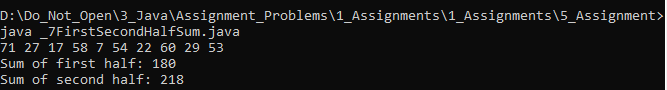
\includegraphics[width=0.8\textwidth]{7.png}
\end{center}

% Problem 8
\section{Exception Handling}
\textbf{Task:} Create a stored procedure \texttt{safe\_add\_employee} that adds an employee 
only if the given department ID exists; otherwise, use \texttt{SIGNAL} to raise 
an error "Invalid Department ID".

\subsection{}
\begin{lstlisting}
DELIMITER //
CREATE PROCEDURE safe_add_employee(IN name VARCHAR(100), IN sal DECIMAL(10,2), IN did INT)
BEGIN
   DECLARE invalid_dept CONDITION FOR SQLSTATE '45000';
   DECLARE EXIT HANDLER FOR invalid_dept
   BEGIN
       SELECT 'Invalid Department ID' AS message;
   END;

   IF (SELECT COUNT(*) FROM departments WHERE dept_id = did) = 0 THEN
       SIGNAL invalid_dept;
   ELSE
       INSERT INTO employees(emp_name, salary, dept_id)
       VALUES (name, sal, did);
       SELECT 'Employee added safely' AS message;
   END IF;
END//
DELIMITER ;

CALL safe_add_employee('Bob', 7000, 1);
CALL safe_add_employee('Charlie', 6000, 99);

\end{lstlisting}

\subsubsection{}
\begin{center}
    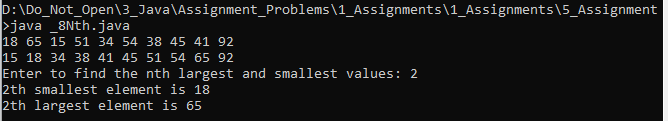
\includegraphics[width=0.8\textwidth]{8.png}
\end{center}

% Problem 9
\section{Exception Handling}
\textbf{Task:} Create a stored procedure \texttt{increase\_salary} that increases salary 
by 10\% for all employees; skip any employees with NULL salary using a \texttt{CONTINUE} handler.

\subsection{}
\begin{lstlisting}
DELIMITER //
CREATE PROCEDURE increase_salary()
BEGIN
   DECLARE done INT DEFAULT 0;
   DECLARE eid INT;
   DECLARE sal DECIMAL(10,2);
   DECLARE cur CURSOR FOR SELECT emp_id, salary FROM employees;
   DECLARE CONTINUE HANDLER FOR NOT FOUND SET done = 1;

   OPEN cur;
   loop1: LOOP
       FETCH cur INTO eid, sal;
       IF done THEN
           LEAVE loop1;
       END IF;

       IF sal IS NULL THEN
           ITERATE loop1;
       END IF;

       UPDATE employees SET salary = salary * 1.10 WHERE emp_id = eid;
   END LOOP;
   CLOSE cur;

   SELECT 'Salaries increased by 10 percent' AS message;
END //
DELIMITER ;

CALL increase_salary();

\end{lstlisting}

\subsubsection{}
\begin{center}
    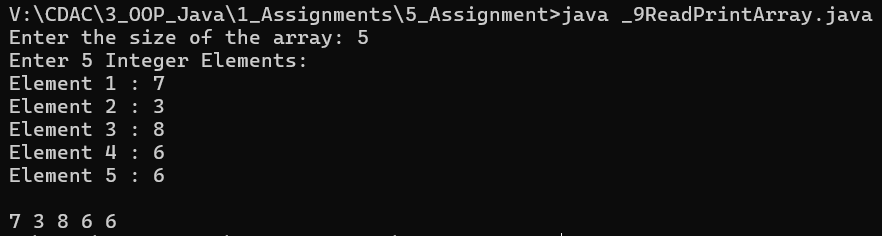
\includegraphics[width=0.8\textwidth]{9.png}
\end{center}

% Problem 10
\section{Exception Handling}
\textbf{Task:} Create a stored procedure \texttt{list\_department\_employees} that lists all employees 
of a given department using a \texttt{CURSOR} and handles the NOT FOUND condition 
gracefully with a \texttt{CONTINUE} handler.

\subsection{}
\begin{lstlisting}
DELIMITER //
CREATE PROCEDURE list_department_employees(IN did INT)
BEGIN
   DECLARE done INT DEFAULT 0;
   DECLARE ename VARCHAR(100);
   DECLARE cur CURSOR FOR SELECT emp_name FROM employees WHERE dept_id = did;
   DECLARE CONTINUE HANDLER FOR NOT FOUND SET done = 1;

   OPEN cur;
   loop2: LOOP
       FETCH cur INTO ename;
       IF done THEN
           LEAVE loop2;
       END IF;
       SELECT ename AS employee_name;
   END LOOP;
   CLOSE cur;
END//
DELIMITER ;

CALL list_department_employees(1);

\end{lstlisting}

\subsubsection{}
\begin{center}
    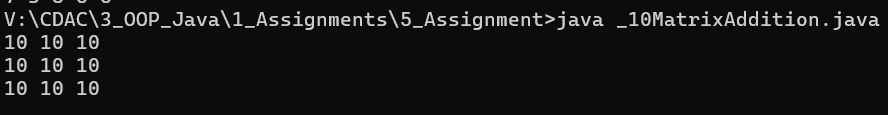
\includegraphics[width=0.8\textwidth]{10.png}
\end{center}

\end{document}
